\documentclass[12pt]{beamer}
\usetheme{Boadilla}
\usepackage{graphicx}
\usepackage{algorithm2e}
\graphicspath{{images/}}
\title{CMPT 155: Computer Applications for Life Sciences}
\subtitle{Lecture 6: Formulas and Functions (Part 2)}
\author{Ivan E. Perez}
\institute{}
\date{January 26, 2022}
\usepackage{booktabs} % Allows the use of \toprule, 
\usepackage{appendix}
\usepackage{enumerate,multicol}
\usepackage{amsmath, amssymb, amsthm}
\usepackage{tikz}
\usepackage{amsxtra}
\begin{document}
	
	\begin{frame}
		\titlepage
	\end{frame}
	
	\begin{frame}
		\frametitle{Presentation Outline}
		\tableofcontents
	\end{frame}
	\section{Homework}
	
	\begin{frame}
		\frametitle{Homework 1}
		\begin{itemize}
			\item Homework 1 will be due next Friday 2/11 6pm. 
			\item No Late Work
			\item Begin \textbf{detail oriented} will be beneficial for the homework.
			\item Having trouble Stop by office hours RLC 204 or join office hours via the google meets link!
		\end{itemize}
	\end{frame}
\section{Conditional Logic}
	\begin{frame}
		\frametitle{Conditional Logic: Order Example}
		\begin{enumerate}
			\item Download \textit{Order.xlsx}
			\item Lets use arithmetic operators to apply a 10\% discount on all orders.
		\end{enumerate}
	it should look like this!
	\begin{center}
		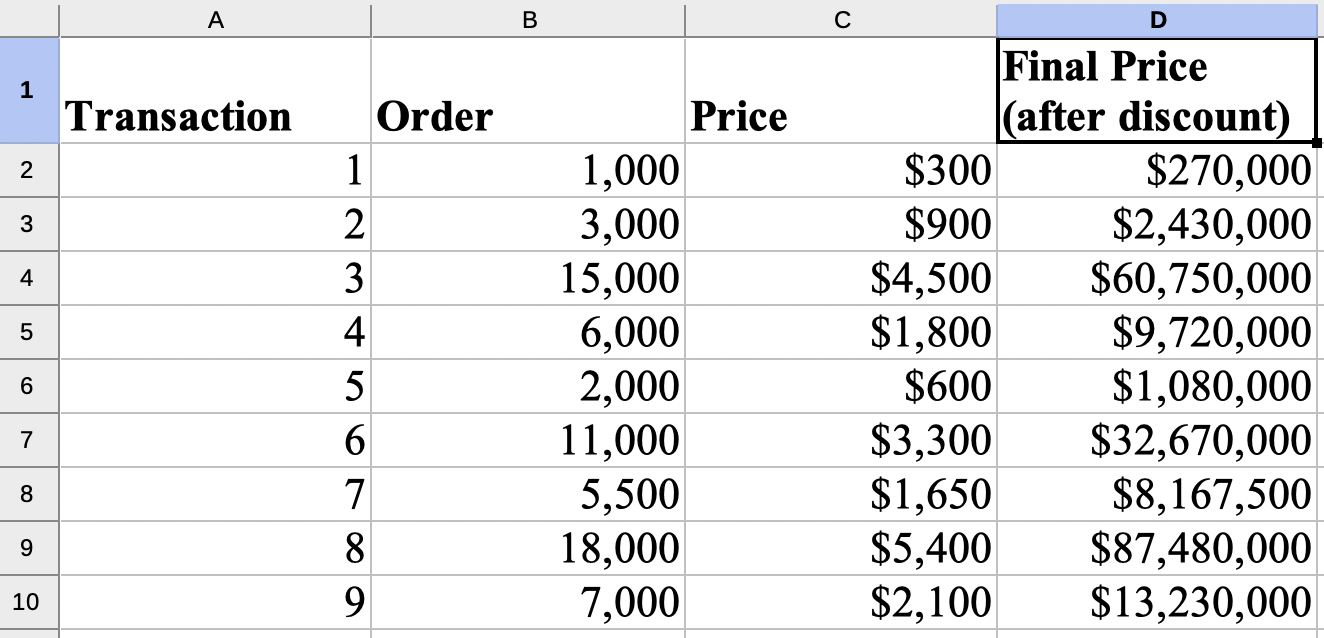
\includegraphics[width=0.5\textwidth]{Order.png}
	\end{center}
	\end{frame}

	\begin{frame}
		\frametitle{Conditional Logic: Order Example Volume Discount}
		We can add conditions to Excel Formulas to return values depending on different logical cases. \\
		Lets try adding a 10\% if the order quantity is over($>$) 5000 units. \\
		It should look like this!
		\begin{center}
			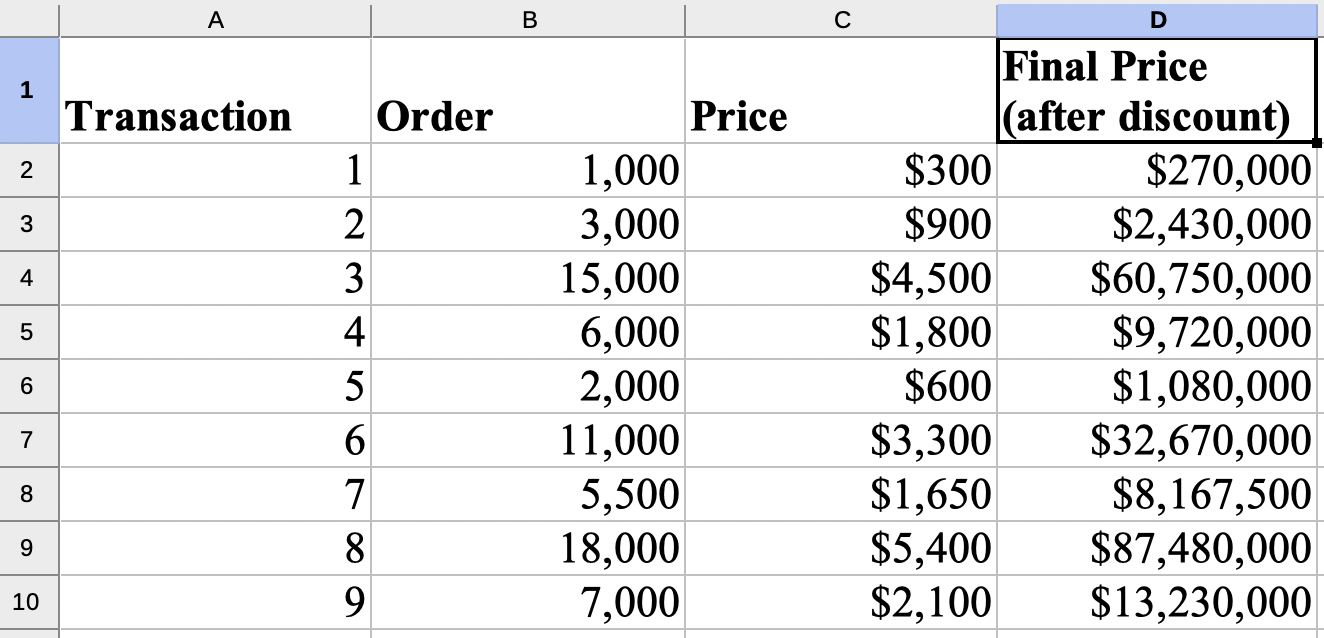
\includegraphics[width=0.5\textwidth]{OrderConditional.png}
		\end{center}
	\end{frame}
	\begin{frame}
		\frametitle{IF()}
		\begin{itemize}
			\item \textbf{IF}(condition, yes\_value, no\_return)
			\item \textbf{How IF() works:}
			\begin{itemize}
				\item  IF takes a logical argument (e.g., $1<2$, $3=4$), and tests whether the argument is \textbf{TRUE}.
				\item  IF the argument is \textbf{TRUE},
				\item THEN value displayed in the cell will be `yes\_value'. \item ELSE it will display the `no\_value'.
			 \end{itemize}
			\item Check out the \textcolor{blue}{ \href{https://support.microsoft.com/en-us/office/if-function-69aed7c9-4e8a-4755-a9bc-aa8bbff73be2}{Microsoft Documentation for IF()}}. 
			\bigskip
			Let's try translating the conditional IF(order is greater than 5000, discounted price, original listed price) into excel!
	\end{itemize}
\end{frame}
\section{Logical Operators}
	\begin{frame}
		\frametitle{Logical Operators}
			\begin{center}
				\begin{tabular}{llll}
					Operator & Name & Example & Return\\
					\hline
					$=$ & Equal to & $1=2$ & FALSE \\
					$>$ & Greater than & $1>2$ & FALSE \\
					$<$ & Less than & $1<2$ & TRUE \\
					$>=$ & Greater than or equal to & $1>=1$ & TRUE\\
					$<=$ & Less than or equal to &  $1<= 1$ & TRUE \\
					$<>$ & Not equal to & $1<>1$ & FALSE
				\end{tabular}
			\end{center}
	\end{frame}
	\begin{frame}
		\frametitle{Exercise 1: Catch Divide by Zero}
		\begin{enumerate}
			\item In cells A1, B1, and C1 write column headers Dividend, Divisor, and Quotient. 
			\item Write the numbers 0,1,2,3,4 in cells A2:A6
			\item in Column B write the numbers -2,1,0,1,2, in cells 
			B2:B6. 
			\item In cells C2:C6 take the quotient. 
			\item what error do we get?
			\item \textbf{Use IF to return the dividend if dividing by 0.} 
		\end{enumerate}
		\begin{center}
		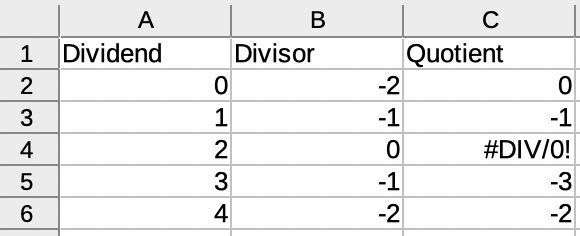
\includegraphics[width= 0.6 \textwidth]{Exercise1Setup.png}
	\end{center}
	\end{frame}
	\begin{frame}
		\frametitle{Exercise 1: Solution}
		\begin{center}
			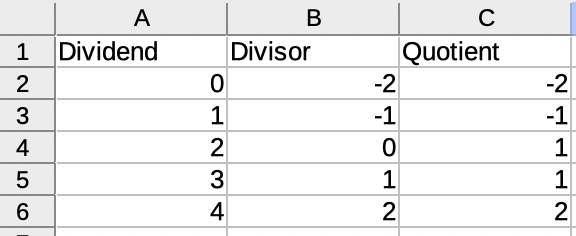
\includegraphics[width= 0.6 \textwidth]{Exercise1Soln.png}
		\end{center}
		\begin{enumerate}
			\item Assuming the setup is correct...
			\item Write `$= \texttt{IF}(\texttt{B2}=0, \text{A2}, \texttt{A2/B2})$'
			\item Use Autofill to apply the formula to cells B3:B6. 
			 
		\end{enumerate}
	\end{frame}
	\begin{frame}
		\frametitle{Exercise 2: Conditional Bonuses}
		\begin{enumerate}
			\item Download `First Quarter Sales and Bonus.xlsx'
			\item Calculate the over target sales.
			\item \textbf{If} the\textit{ over target sales} \textbf{greater than} \textit{\texttt{0}}, then the sales man gets a 5\% commision (based on the \textit{over target sales}). 
			\item Calculate the total salary.   
		\end{enumerate}
	\end{frame}
	\begin{frame}
		\frametitle{Exercise 2: Solution}
		\begin{itemize}
			\item In cell E4, take the difference between C4 and D4.
			\item To handle negative over target sales:\begin{enumerate}
				\item use IF() to change negative overtarget sales to 0. 
				\item it should be =IF($\texttt{D4}-\texttt{C4}< 0, 0, \texttt{D4} -\texttt{C4}$)
				\end{enumerate}
			\item Use Autofill to apply the difference to cells E5:E12. 
			\item In cell F4, calculate the 5\% comission bonus by mutiplying the `over target sales', E4, by 0.05. 
			\item Use Autofill to calculate the overtarget sales for each salesman. 
			\item In cell H4, calculate the sum between E4 and F4.
			\item Use Autofill to calculate the sum for each salesman. 
		\end{itemize}
	\end{frame}
	\begin{frame}	
		\frametitle{Exercise 2: Solution Table}
		\begin{figure}
			\begin{center}
				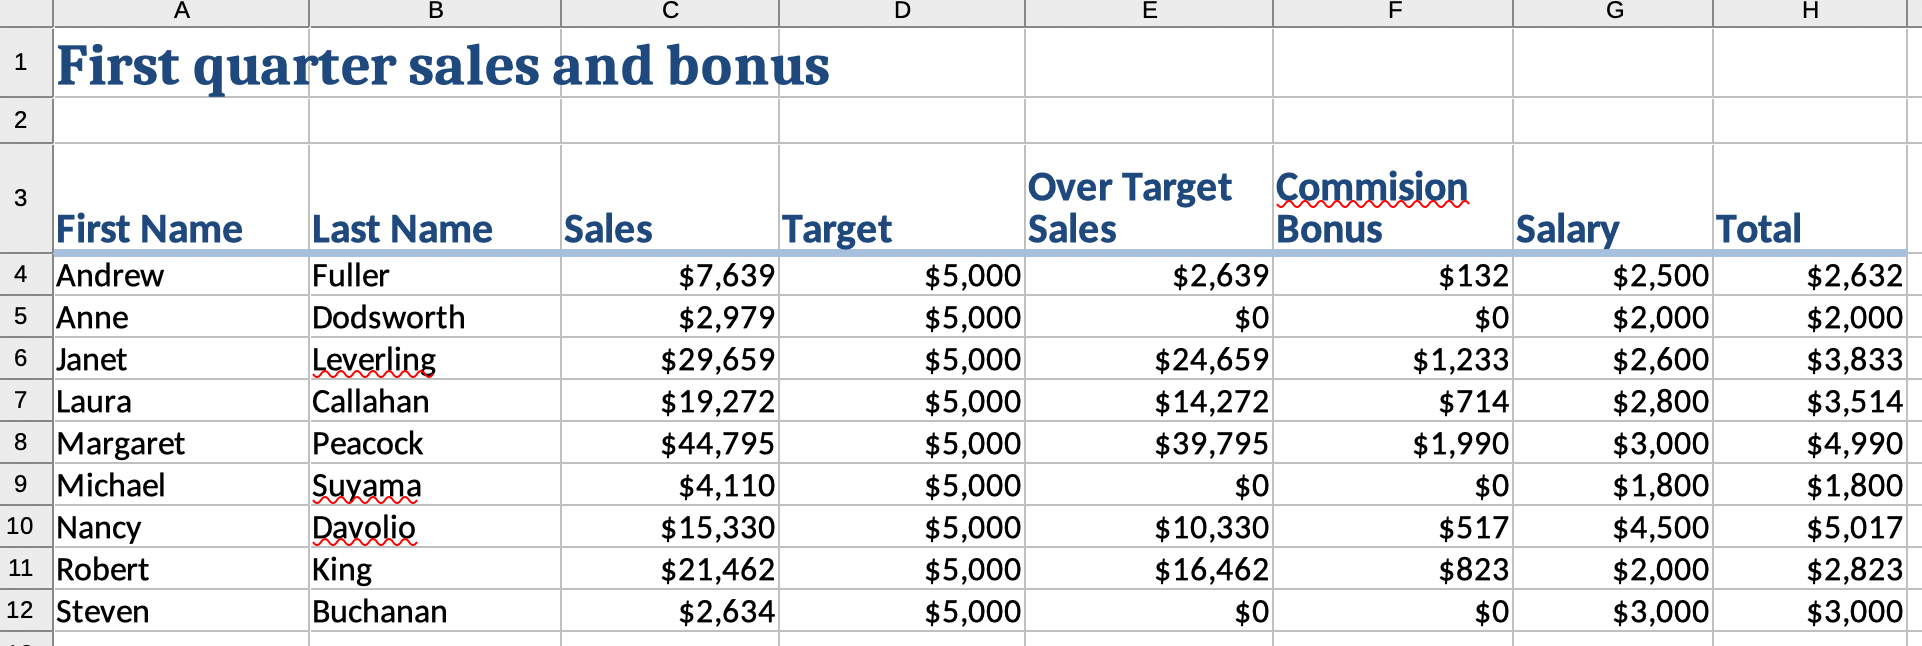
\includegraphics[width=\textwidth]{Exercise2Soln.png}
			\end{center}
			\caption{First Quarter Sales and Bonus}
		\end{figure}
	\end{frame}
\section{Functions and Formulas}
	\begin{frame}
		\frametitle{Exercise 3: Fruit Purchase}
		\begin{enumerate}
			\item Download Fruit\_Purchase.xlsx
			\item Count the occurrences of each fruit. 
		\end{enumerate}
	\end{frame}
	\begin{frame}
		\frametitle{Exercise 3: Solution}
		\begin{enumerate}
			\item In Cells C2, D2, and E2 write the following column headers; `Is Apple?', `Is Kiwi?', `Is Pear?'. 
			\item Logical Tests
			\begin{enumerate}
				\item Check if the corresponding cell matches the Fruit in question.
				\item For apples; In Cell C3, type $=\texttt{IF}(\texttt{B3} = \texttt{"apples"}, 1, 0)$
			\end{enumerate}
		\item Use Autofill from Cell C3 to apply the logical test down each Column. 
		\item In Cell B22 use SUM() to sum all the occurences of apples by writing =SUM(C3:C20).
		\item Repeat Steps 2-4, for each fruit (Note: Be careful to type the fruit exactly as written). 
		\end{enumerate}
	\end{frame}

	\begin{frame}
		\frametitle{Exercise 3: Solution}
		\begin{center}
			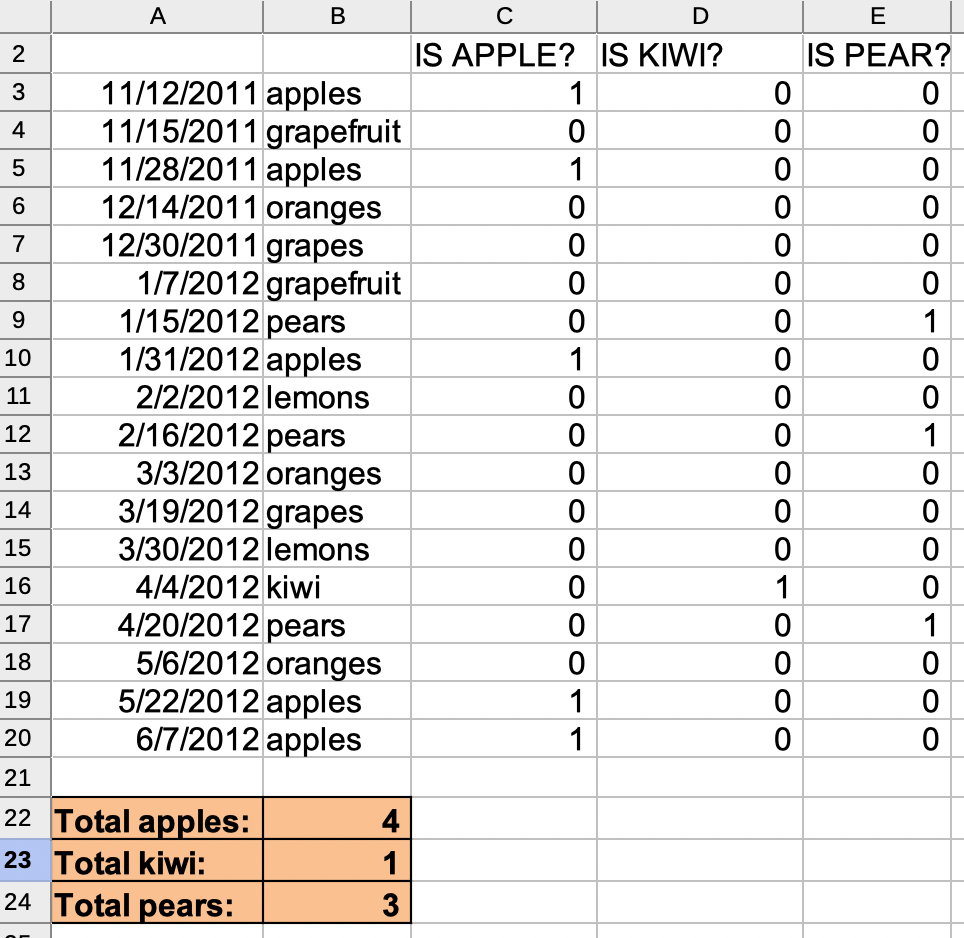
\includegraphics[width=0.7\textwidth]{Exercise3Soln.png}
		\end{center}
	\end{frame}
\section{Absolute Cell References}
	\begin{frame}
		\frametitle{Absolute Cell References}
		Up to now we have used Autofill to sequentially apply formulas down a column. 
		Sometimes we want to  \textbf{Lock} a cell reference so that it is used in multiple calculations!
		
		To \textbf{Lock} a:
		\begin{itemize}
			\item Column while applying a function across a Row.
			\begin{itemize}
				\item Type a \$ in front of the column reference (e.g., A\$1).
			\end{itemize}
			\item Row while applying a function down a Column.
				\begin{itemize}
				\item Type a \$ in front of the row reference (e.g., \$A1).
				\end{itemize}
			\item Both Columns and Rows: 
				\begin{itemize}
					\item Type \$ in front of both (e.g., \$A\$1)
					\item when in doubt just use both!
				\end{itemize}
			\end{itemize}
			\end{frame}
	\begin{frame}
		\frametitle{Exercise 4: Student Grades 2}
		\begin{enumerate}
			\item Download \textit{ StudentGrades2.xlsx}
			\item Use absolute cell references to calculate the Final Score for each student.
			\item Calculate the Total and Average Final Score. 
			\item BONUS: Try to find the Median, Minimum, and Max Scores.  
		\end{enumerate}
	\end{frame}
	\begin{frame}
		\frametitle{Exercise 4: Solution}
		\begin{enumerate}
			\item In Cell E2, Calculate the individual percentage scores for each assignment using absolute cell references.
			\item Separate each score by a `+' sign to take an unweighted sum.
				\begin{itemize}
					\item cell E2 should read\\ \texttt{=(B2/\$B\$12) + (C2/\$C\$12) + (D2/\$D\$12)}
				\end{itemize}
			\item Get a weighted average by multiplying each score by its associated weight. 
				\begin{itemize}
					\item cell E2 should finally read\\ \texttt{=0.25*(B2/\$B\$12) + 0.25*(C2/\$C\$12) + 0.5*(D2/\$D\$12)}
				\end{itemize}
				\item Use Autofill to generate scores for each student.
				\item In cell E14, use SUM() over cells E2:E10. 
				\item In cell E15, use Average over cells E2:10.
		\end{enumerate}
	\end{frame}
	\begin{frame}
		\frametitle{Exercise 4: Solution}
		\begin{enumerate} \item Select cells A2:E10
			\item click Home $\rightarrow$ Sort \& Filter $\rightarrow$ Custom Sort...
			\item In the Sort dialog box Select Column E as the Sort Column. 
			\item Select Smallest to Largest as the sort order.
			\item In cell E16 enter the reference for the median E6.
			\item In cell E17 enter the cell reference for the highest score E10.
			\item In cell E18 enter the cell reference for the second highest score .
			\item In cell E19 enter the cell reference for the lowest score E2.
		\end{enumerate}
	\end{frame}
	\begin{frame}
		\frametitle{Exercise 4: Solution Continued}
		\begin{center}
			\includegraphics[width=0.9\textwidth]{Exercise4Soln.png}
		\end{center}
	\end{frame}
	\section{AND() Function, \& Nested Functions}
	\begin{frame}
	\frametitle{AND() Function}
	\begin{itemize}
	\item AND() accepts two (or more) conditions, and then returns true if all of them are true.
	\item If any condition is false, AND() returns false. 
	\item e.g., the new commission rules (5\% rate)
	came into effect after the year 2010. 
	\item \texttt{= IF( AND(E6>0, F6>2010), E6*0.05, 0)}
	\end{itemize}	
\end{frame}
\begin{frame}
	\frametitle{Exercise 5: Student Grades 3}
	\begin{enumerate}
		\item Download \textit{StudentGrades3.xlsx}
		\item Let the student only pass if they pass \textbf{BOTH} tests with a score of \textbf{at least} 60. 
		\item Use conditional formatting to highlight the failed ones in yellow. 
	\end{enumerate}
\end{frame}
\begin{frame}
	\frametitle{Exercise 5: Solution}
	\begin{enumerate}
		\item In Cell D2 start an IF() statment.
		\item in the IF statmemt begin an AND() statement.
		\item In the AND() function write the following logical tests separated by a column.
		\begin{itemize}
			\item $\texttt{B2}>=60$ 
			\item $\texttt{C2}>=60$
		\end{itemize}
		\item in the second and third arguments write ``FAIL", and ``PASS" respectively, to return the correct result 
		\begin{itemize}
			\item Cell D2 should read\\
			\texttt{=IF(AND(B2>=60, C2 >= 60), "PASS", "FAIL")} 
		\end{itemize}
		\item Use Autofill to check the scores for each student.
		\item Select the cells D2:D10 and apply the conditional formatting.
	\end{enumerate}
\end{frame}
\begin{frame}
	\frametitle{OR() Function}
	\begin{itemize}
	\item accepts two (or more) conditions, and then returns true if any one of them is true.
	\item OR() returns false only if all conditions are false.
	\item = IF (OR(condition 1, condition 2), value\_if\_true, value\_if\_false)
	\end{itemize}
\bigskip
Try it on \textit{StudentGrades3}!
\end{frame}
\begin{frame}
	\frametitle{Exercise 5: Solution Continued}
	\begin{center}
		\includegraphics[width=0.8\textwidth]{Exercise5Soln.png}
	\end{center}
\end{frame}
\begin{frame}
	\frametitle{Exercise 6: Fruit Purchases Redux}
	\begin{enumerate}
		\item Download \textit{Fruit\_Purchase.xlsx}
		\item In Column C Insert a column named ``Is Citrus?". 
		\item Use  SUM(), IF() and OR() to count the number of Fruits that could be classified as a Citrus (e.g., grapefruit, orange, lemon).
		\item place this result in Cell B25.
	\end{enumerate}
\end{frame}
\begin{frame}
	\frametitle{Exercise 6: Solution}
	\begin{enumerate}
		\item begin by adding a column header ``Is Citrus" in Cell C2.
		\item In cell A25 add a total label ``Total Citrus".
		\item In cell C3 start an if statment followed by an OR statement.
			\begin{itemize}
				\item The cell should read \\
				\texttt{=IF(OR(}
			\end{itemize}
		\item Write the three logical tests separated by columns.
			\begin{itemize}
				\item The cell should now read \\
				\texttt{=IF(OR(B3="grapefruit", B3="lemons", B3="oranges")}
			\end{itemize}
		\item since we are interested in counting the instances where this statement is true, the TRUE and FALSE return statments should be 1, 0 respectively.
			\begin{itemize}
				\item Cell C3 should finally read \\
				\texttt{=IF(OR(B3="grapefruit", B3="lemons", B3="oranges"), 1, 0)}
			\end{itemize}
	\item use autofill to fill out the columns C3:C20.
	\item In Cell B25 sum the values in the selection C3:C20.
		\begin{itemize}
			\item Cell B25 should read \texttt{=SUM(C3:C20)}
		\end{itemize}
	\end{enumerate}
\end{frame}
\begin{frame}
	\frametitle{Exercise 6: Solution Continued}
	\begin{center}
		\includegraphics[width=0.6\textwidth]{Exercise6Soln.png}
	\end{center}
\end{frame}
\begin{frame}
	\frametitle{NOT()}
	\begin{itemize}
		\item NOT() accepts a condition and reverse it. 
		\begin{itemize}
			\item \texttt{= IF ( NOT(B2>0), ........ , ......... )}
		\end{itemize}
	\end{itemize}
Example! Try applying the NOT() statement by replicating the table below:
\begin{center}
	\begin{tabular}{l | l | l }
	Statement & T/F  & NOT(T/F)\\ 
	\hline
	1=2 & FALSE & TRUE \\
	2>1  & TRUE & FALSE \\ 
	10<=3 & FALSE & TRUE 
	\end{tabular}
\end{center}
Your table should be entered in this fashion:
\begin{center}
	\begin{tabular}{l |l | l}
		Statement & T/F  & NOT(T/F)\\ 
		\hline
		1=2 & \texttt{=1=2} & \texttt{=NOT(1=2)} \\
		2$>$1  & \texttt{=2>1}& \texttt{=NOT(2>1)}\\ 
		10$<=$3 & \texttt{=10>=3} & \texttt{=NOT(10>=3)}
	\end{tabular}
\end{center}
\end{frame}

\end{document}

% things to do 
% pics replace, notes




